%%%%%%%%%%%%%%%%%%%%%%%%%%%%%%%%%%%%%%%%%%%%%%%%%%%%%%%%%%%%%%%%%%%%%%%%%%%%%
%	e-Yantra, IIT-Bombay

%	Document Author: Abhishek Rathore, Gopineedi Harsha Vardhan
%	Date: 07-June,2016 

%%%%%%%%%%%%%%%%%%%%%%%%%%%%%%%%%%%%%%%%%%%%%%%%%%%%%%%%%%%%%%%%%%%%%%%%%%%%%

\documentclass[11pt,a4paper]{article}

\usepackage{graphicx}
\usepackage{listings}
\usepackage{url}
\usepackage{float}
\usepackage{subcaption}
\usepackage{hyperref}
\title{Tutorial on CAMShift Algorithm and How to use it using OpenCV and Python for Object Tracking}
\author{e-Yantra Team}
\date{\today}

\begin{document}
	\maketitle
	\newpage
	\tableofcontents
	\newpage
	\section{Objective}
		The objective of this tutorial is to describe the working of "Continuously Adaptive Meanshift (Camshift) Algorithm" and to explain "How to use this algorithm in OpenCV and Python for Object Tracking"
	\section{Prerequisites}
		User should have handy knowledge of following before reading this tutorial.
		\begin{itemize}
			\item Basics of Python Language.
			\item Introduction to OpenCV.
			\item Basics of Image processing in OpenCV using Python.
			\item Knowledge on Mean Shift Algorithm,Histograms and Back projections.
		\end{itemize}
	\section{Hardware Requirement}
		\begin{itemize}
			\item A Computer with internal or external webcam.
		\end{itemize}
	\section{Software Requirement}
		\begin{itemize}
			\item Python 2.7.5 (with OpenCV and Numpy module)
			\item OpenCV 2.4.9 
			\item numpy 1.7.1
			\item Any sample video(that can be used for object tracking)
			\item \textbf{Note :} These versions I had at the time of this tutorial.
		\end{itemize}
	\section{Theory and Description}
		The full form of Camshift Algorithm is Continuously Adaptive Meanshift Algorithm and it is improved version of Meanshift Algorithm. So it is good to understand Meanshift Algorithm before Camshift algorithm to get better idea of Camshift algorithm.
		\subsection{Meanshift Algorithm}
			Meanshift is a non-parametric feature-space analysis technique, a so-called mode seeking algorithm. It is a procedure for locating the maxima of a density function given discrete data sampled from that function. In a sense, it is using a non-parametric density gradient estimation. It is useful for tracking the objects.
			
			Moving objects are characterized by their color-histograms. Therefore the key operation of the object tracking algorithm is histogram estimation. Meanshift tracking algorithm is an iterative scheme based on comparing the histogram of the original object in the current image frame and histogram of candidate regions in the next image frame. 
			 
			The aim is to maximize the correlation between two histograms.Object tracking for an image frame is performed by a combination of histogram extraction, weight computation and derivation of new location. 
			
			Consider you have a set of points as given in Figure 1. (It can be a pixel distribution like histogram backprojection). You are given a small window (may be a circle) and you have to move that window to the area of maximum pixel density (or maximum number of points). It is illustrated in the Figure 1.
			\begin{figure}[h!]
				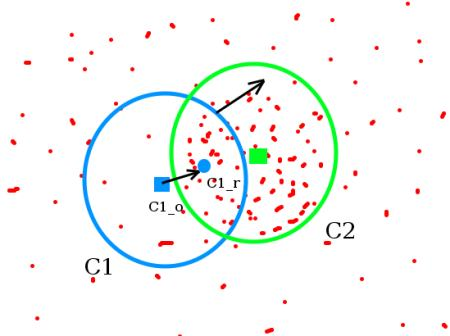
\includegraphics[scale=0.5 ]{../Images/meanshift.jpg}
				\centering
				\caption{Meanshift Algortithm (Courtesy: opencv-python-tutroals.readthedocs.io)}
			\end{figure}
			
			The initial window in Figure 1 is shown in blue circle with the name “C1”. Its original center is marked in blue rectangle, named “C1.o”. But if you find the centroid of the points inside that window, you will get the point “C1.r” (marked in small blue circle) which is the real centroid of window. Surely they don’t match. So move your window such that circle of the new window matches with previous centroid. Again find the new centroid. Most probably,it won’t match. So move it again, and continue the iterations such that center of window and its centroid falls on the same location (or with a small desired error). So finally what you obtain is a window with maximum pixel distribution. It is marked with green circle, named “C2”.
			
			But the major drawback of meanshift algorithm is that it does not changes the size and orientation of the track window of the object with respect to scale and orientation of the object. It was removed in Camshift Algorithm, which is described below.
		\subsection{Camshift Algorithm}
			Camshift algorithm is an improvement of Meanshift algorithm known as Continously Adaptive Mean shift algorithm.It applies meanshift first.Once meanshift converges, it updates the size of the window using formula given in figure 2 and M00 is zeroth moment of track window.
			\begin{figure}[h!]
				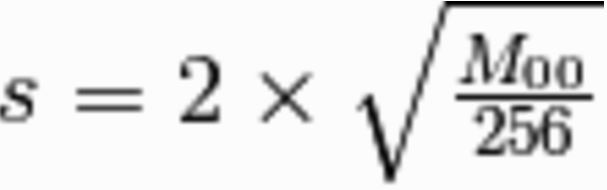
\includegraphics[scale=0.5 ]{../Images/scale_estimation.JPG}
				\centering
				\caption{Formula (Courtesy: opencv-python-tutroals.readthedocs.io)}
			\end{figure}
			
			It also calculates the orientation of best fitting ellipse to it. Again it applies the meanshift with new scaled search window and previous window location. The process is continued until required accuracy is met.
			
			It is almost same as meanshift, but it returns a rotated rectangle (that is our result) and box parameters (used to be passed as search window in next iteration).
			
			The Camshift cleverly exploits the algorithm of mean-shift by changing the size of the window when it happened to convergence. The Camshift coupled is an adaptation to the color image sequences, and is operated in pursuit of real-time object.
			
			\subsubsection{Illustration of Camshift algorithm in a Second video frame}
				Let in first frame face was inside red rectangle (shown in Figure 3(a)) so it was selected as Region of Interest in first frame. And in Second frame, let face moves from previous position and comes the position as shown in Figure 3(a). So at first Camshift algorithm calculates mean of white pixels in back projection of frame. Then it makes mean as the new center of the window as shown, it is called meanshift iteration in Camshift Algorithm. Meanshift first iteration is shown in Figure 3(a). Meanshift second iteration , third iteration and convergence of Meanshift is shown in figure 3
				\begin{figure}[h!]
					\begin{subfigure}{0.5\textwidth}
						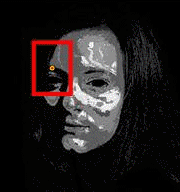
\includegraphics[width=0.9\linewidth, height=3.8cm]{../Images/msi.png} 
						\caption{Meanshift 1st iteration}
					\end{subfigure}
					\begin{subfigure}{0.5\textwidth}
						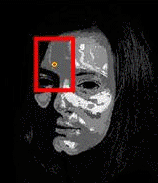
\includegraphics[width=0.9\linewidth, height=3.8cm]{../Images/ms2nd.png}
						\caption{Meanshift 2nd iteration}
					\end{subfigure}
					\begin{subfigure}{0.5\textwidth}
						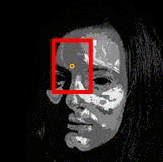
\includegraphics[width=0.9\linewidth, height=3.8cm]{../Images/ms3rd.png}
						\caption{Meanshift 3rd iteration}
					\end{subfigure}
					\begin{subfigure}{0.5\textwidth}
						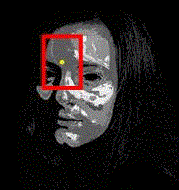
\includegraphics[width=0.9\linewidth, height=3.8cm]{../Images/msconverged.png} 
						\caption{Converged  Meanshift}
					\end{subfigure}
					\caption{Courtesy: opencv-python-tutroals.readthedocs.io}
				\end{figure}
				
				Then it calculates size of the window according to formula given in Figure 2 as shown in Figure 4(a). Then if finds minimum area ellipse to give the orientation of object as shown in Figure 4(b). And this process continues iteratively as shown in Figure 4(c) and Figure 4(d). 
				\begin{figure}[h!]
					\begin{subfigure}{0.5\textwidth}
						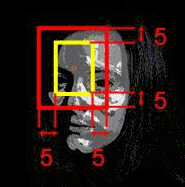
\includegraphics[width=0.9\linewidth, height=3.8cm]{../Images/roiforellipse.png}
						\caption{Calculation of roi}
					\end{subfigure}
					\begin{subfigure}{0.5\textwidth}
						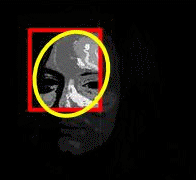
\includegraphics[width=0.9\linewidth, height=3.8cm]{../Images/ellipsecomputation.png}
						\caption{Ellipse computation}
					\end{subfigure}
					\begin{subfigure}{0.5\textwidth}
						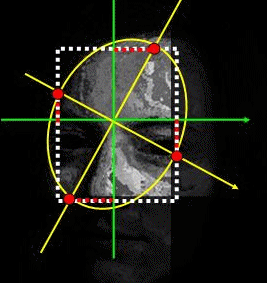
\includegraphics[width=0.9\linewidth, height=3.8cm]{../Images/newmeanshiftaxis.png} 
						\caption{New meanshift axis}
					\end{subfigure}
					\begin{subfigure}{0.5\textwidth}
						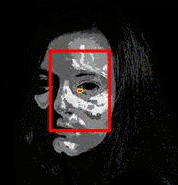
\includegraphics[width=0.9\linewidth, height=3.8cm]{../Images/meanshiftagain.png}
						\caption{Meanshift again}
					\end{subfigure}
					\caption{ellipse computation and applying Meanshift again (Courtesy: opencv-python-tutroals.readthedocs.io)}
				\end{figure}
				
				After convergence it calculates converged ellipse as shown in Figure 5.
				\begin{figure}[h!]
					\begin{subfigure}{0.5\textwidth}
						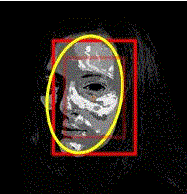
\includegraphics[width=0.6\linewidth, height=3cm]{../Images/msec.png} 
						\caption{Ellipse calculation}
					\end{subfigure}
					\begin{subfigure}{0.5\textwidth}
						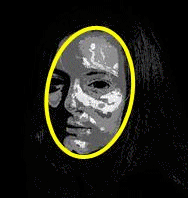
\includegraphics[width=0.6\linewidth, height=3cm]{../Images/convergedellipse.png}
						\caption{Converged Ellipse}
					\end{subfigure}
					\caption{Converged ellipse calcualtion (Courtesy: opencv-python-tutroals.readthedocs.io)}
				\end{figure}
				
				Camshift result is shown in Figure 6
				\begin{figure}[h!]
					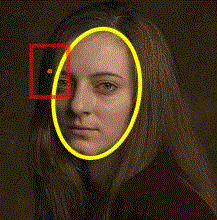
\includegraphics[scale = 0.5]{../Images/result.png}
					\centering
					\caption{Resulting Camshift (Courtesy: opencv-python-tutroals.readthedocs.io)}
				\end{figure}
		\newpage
		\subsection{Using Camshift Algorithm using Python OpenCV}
			To use Camshift Algorithm in OpenCV and Python following steps are required.
			\begin{itemize}
				\item After getting Region of Interest, we mask it for better result.
				\item We get 2D histogram of ROI using inbuilt OpenCV function cv2.calcHist().
				\item We normalize histogram in the range 0 to 1 using OpenCV function cv2.normalize.
				\item Initial ROI operattions is shown in Figure 7
				\begin{figure}[h!]
					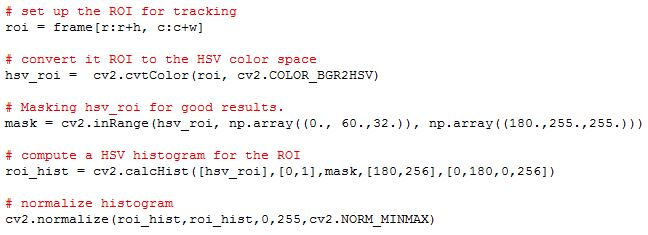
\includegraphics[scale=0.8 ]{../Images/roi_code.JPG}
					\centering
					\caption{Initial ROI operations}
				\end{figure}
				\item Then in the next frame, color space is changed from RGB to HSV using OpenCV function cv2.cvtColor().
				\item It extracts object by back projecting ROI in current frame using ROI histogram.
				\item New bounding box, and minimum area rectangle is found using OpenCV inbuilt function cv2.CamShift() which uses back projection, previous bounding box, and termination criteria.
				\item code for frame operation is shown in Figure 8.
				\begin{figure}
					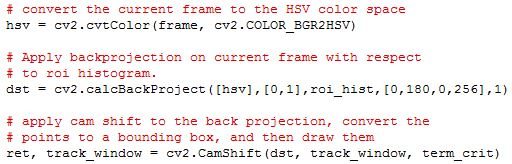
\includegraphics[scale=0.8 ]{../Images/frame_code.JPG}
					\centering
					\caption{Frame operations}
				\end{figure}
				\newpage
				\item It draws rotating rectangle using output of cv2.CamShift(), 'ret'.
				\item Drawing of rectangle is shown in figure 9.
				\begin{figure}
					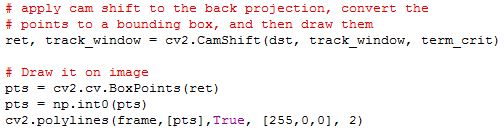
\includegraphics[scale=0.8 ]{../Images/drawing_code.JPG}
					\centering
					\caption{Drawing operations}
				\end{figure}
				\item This process will run iteratively.
			\end{itemize}
	\section{Code}
		The Python code using OpenCV and Numpy can be found \href{https://github.com/eYSIP-2016/Object-Tracking-Camera/tree/master/Tutorials/2.%20Tutorial%20on%20CAMShift%20Algorithm%20and%20How%20to%20use%20it%20using%20OpenCV%20and%20Python%20for%20Object%20Tracking/Code}{here}.
		Step to use code are as shown below.
		\begin{itemize}
			\item Download and run code using Python Idle.
			\item press space bar to pause the video and give bounding box using mouse drag and drop.
			\item press space bar to track object.
		\end{itemize}
	
	\section{Exercise}
		Real time object tracking in a sample video is shown in Figure 10 and Figure 11.          
		\begin{figure}[h!]
			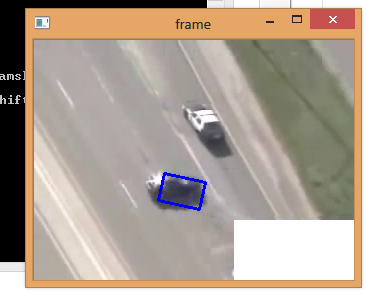
\includegraphics[scale=1.1]{../Images/Vid_ROI.png}
			\centering
			\caption{Selecting suspect car in a chase as ROI (Courtesy: youtube.com)}
		\end{figure}
		\begin{figure}[h!]
			 \includegraphics[scale=1.1]{../Images/Vid_Det.png}
			 \centering
			 \caption{Tracking the suspect in the frame (Courtesy: youtube.com)}
		\end{figure}
		\newpage
		Real time object tracking in a webcam is shown in Figure 12 and Fig 13.  
		\begin{figure}[h!]
			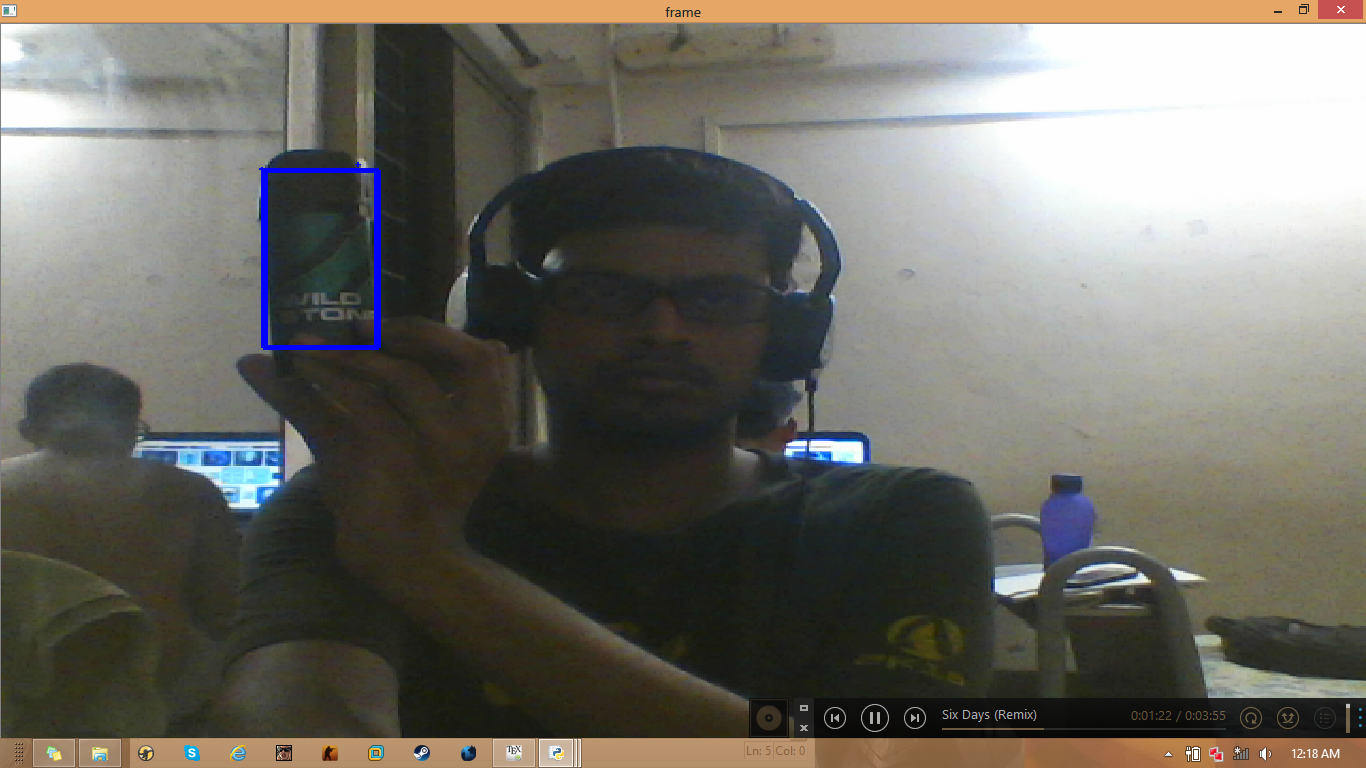
\includegraphics[width=0.9\linewidth, height=6.8cm]{../Images/Cam_ROI.png}
			\centering
			\caption{Selecting Deodrant as ROI}
		\end{figure}
		\begin{figure}[h!]
			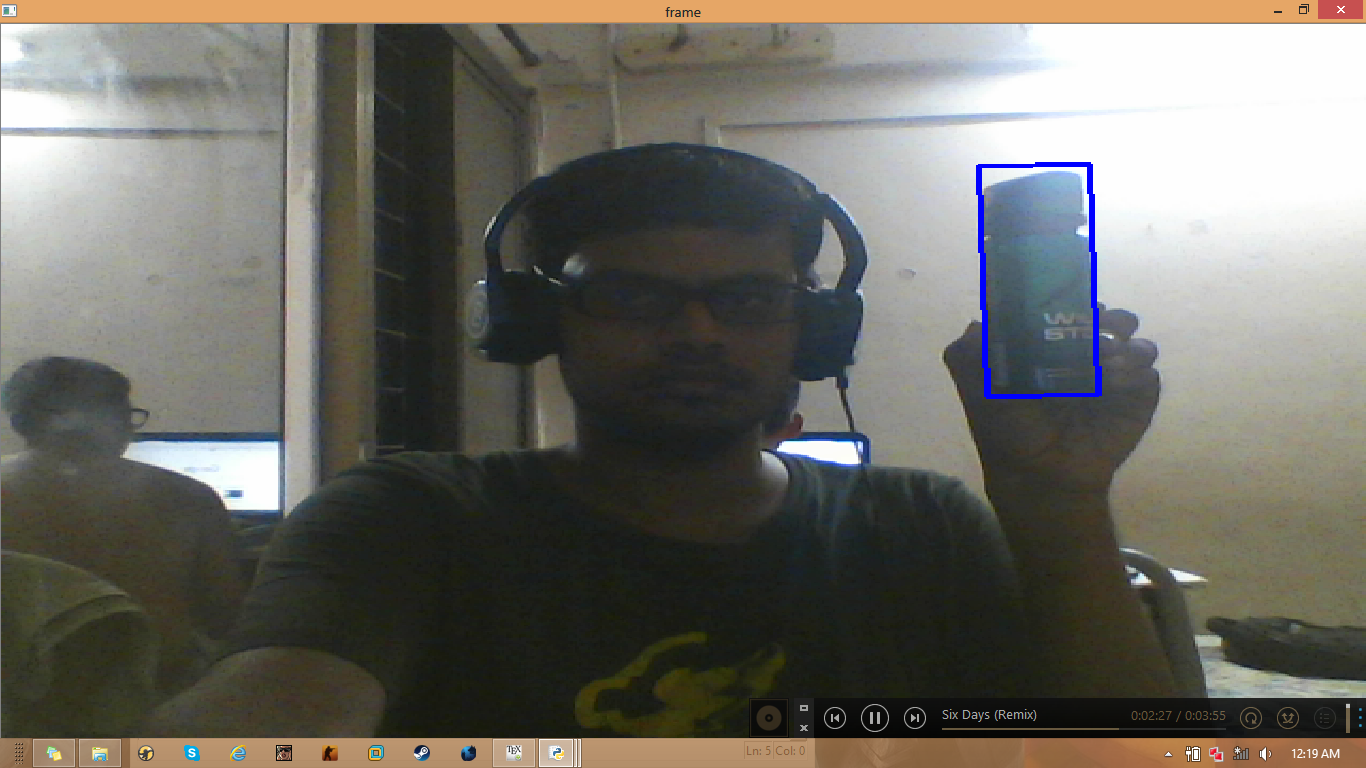
\includegraphics[width=0.9\linewidth, height=6.8cm]{../Images/Cam_Det.png}
			\centering
			\caption{Tracking the Deodrant in the frame}
		\end{figure}
	
	\newpage
	\section{References}
		\begin{enumerate}
			\item \url{http://opencv-python-tutroals.readthedocs.io/en/latest/py_tutorials/py_video/py_meanshift/py_meanshift.html#meanshift}
			\item \url{http://www.bogotobogo.com/python/OpenCV_Python/python_opencv3_mean_shift_tracking_segmentation.php}
			\item \url{http://www.computervisiononline.com/blog/tutorial-using-camshift-track-objects-video}
			\item \url{https://sites.google.com/a/ualberta.ca/jinxin-he/programming/python/simpleobjecttracking}
			\item \url{http://www.pyimagesearch.com/2015/05/25/basic-motion-detection-and-tracking-with-python-and-opencv/}
		\end{enumerate}
			
\end{document}



